\opsim~and \altsched~schedulers have adopted two different ways of observing the sky. While the former relies on a greedy algorithm to decide which pointing should be performed (optimisation based on slew-time minimisation, optimal observing conditions - in terms of sky brightness and airmass for instance), the latter scans near the meridian dense areas (pre-defined at the begining of the night) of the sky. Fig. \ref{fig:night_comp} illustrate the area observed at the end of a night for both schedulers. One may observe that \altsched~scans dense area of the sky while regions observed by \opsim~are sparsely populated. It may thus be more difficult to ensure a regular cadence with \opsim~method. Both schedulers perform observations near the meridian (Fig. \ref{fig:scan_meridian}).

\begin{figure}[!htbp]
  \centering
  \subfigure[OpSim]{\label{fig:opsim_night}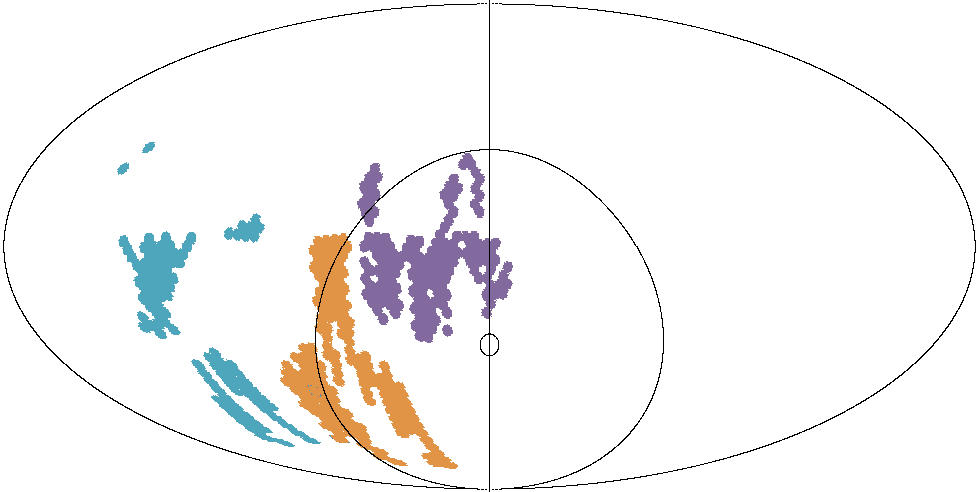
\includegraphics[width=0.8\textwidth]{opsim_vs_altsched/opsim_night.png}}
  \subfigure[altsched]{\label{fig:altsched_night}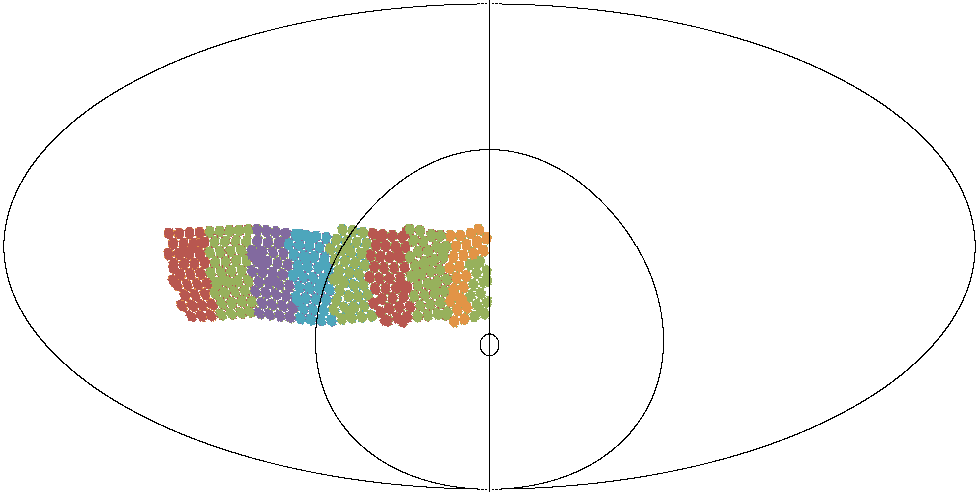
\includegraphics[width=0.8\textwidth]{opsim_vs_altsched/altsched_night.png}}
  \caption{Area coverage at the end of a night for \opsim(top) and \altsched(bottom) schedulers.  Each color point corresponds to a pointing. Colors correspond to the latest filter used.}\label{fig:night_comp}
\end{figure}

\begin{figure}[!htbp]
  \begin{center}
    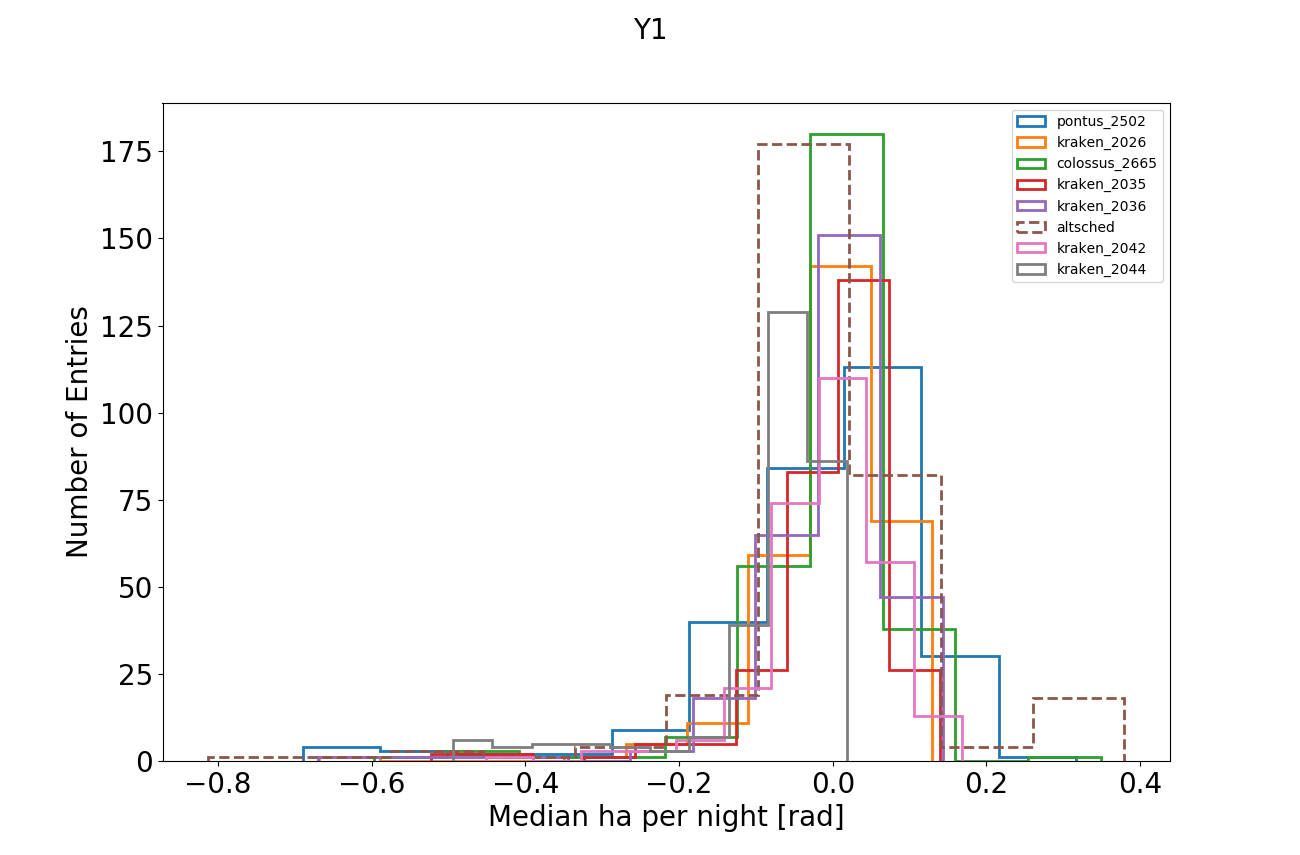
\includegraphics[width=0.6\textwidth]{opsim_vs_altsched/median_ha.png}
    \caption{Median hour angle (first year of the survey) for some of the observing strategies considered in this work.}\label{fig:scan_meridian}
    \end{center}
\end{figure}

One may also observe on Fig. \ref{fig:night_comp} that the filter allocation is quite different between the two schedulers during a night. The number of filter changes per night is indeed higher for \altsched(median value: 12) compared to \opsim(median value: 2) as it can be seen on Fig. \ref{fig:filter_changes}. The global filter allocation (ie the fraction of visits per band after ten years) with \altsched~is not the same in \opsim (see Appendix \ref{sec:globalstat}): in comparison to \opsim~, \altsched~tends to allocate a larger (lower)  number of visits in [u,g,r,z] ([i,y]) bands. This has an impact on \sne~observations in the WFD survey since [g,r,i] are the bands of interest for the redshift range ($z \lesssim 0.4$) accessible.

\begin{figure}[!htbp]
  \begin{center}
    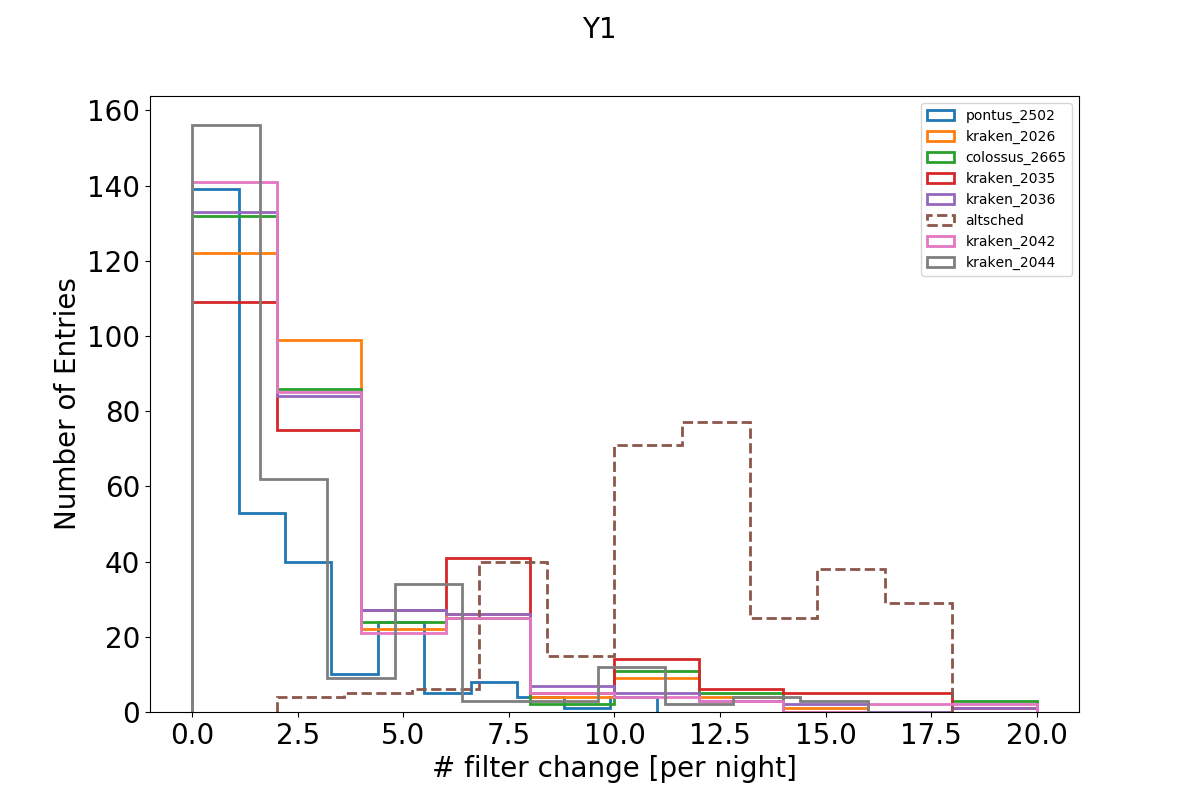
\includegraphics[width=0.6\textwidth]{opsim_vs_altsched/filter_changes.png}
    \caption{Number of filter changes per night (first year of the survey) for some of the observing strategies considered in this work.}\label{fig:filter_changes}
    \end{center}
\end{figure}

A common criticism on \altsched~is that this scheduler allows observations (except in the u-band) when the distance to the Moon is low. While this is true (Fig. \ref{fig:moondist}) one may consider that this correspond to up to ten percent of the total number of visits and that the Moon distance constraint (cut at 30 degrees in \opsim~) may be included in a quite easy way in the code. It would be interesting to run \altsched~simulations including the Moon distance constraint so as to evaluate potential impacts on cadence and filter allocation.

\begin{figure}[!htbp]
  \begin{center}
    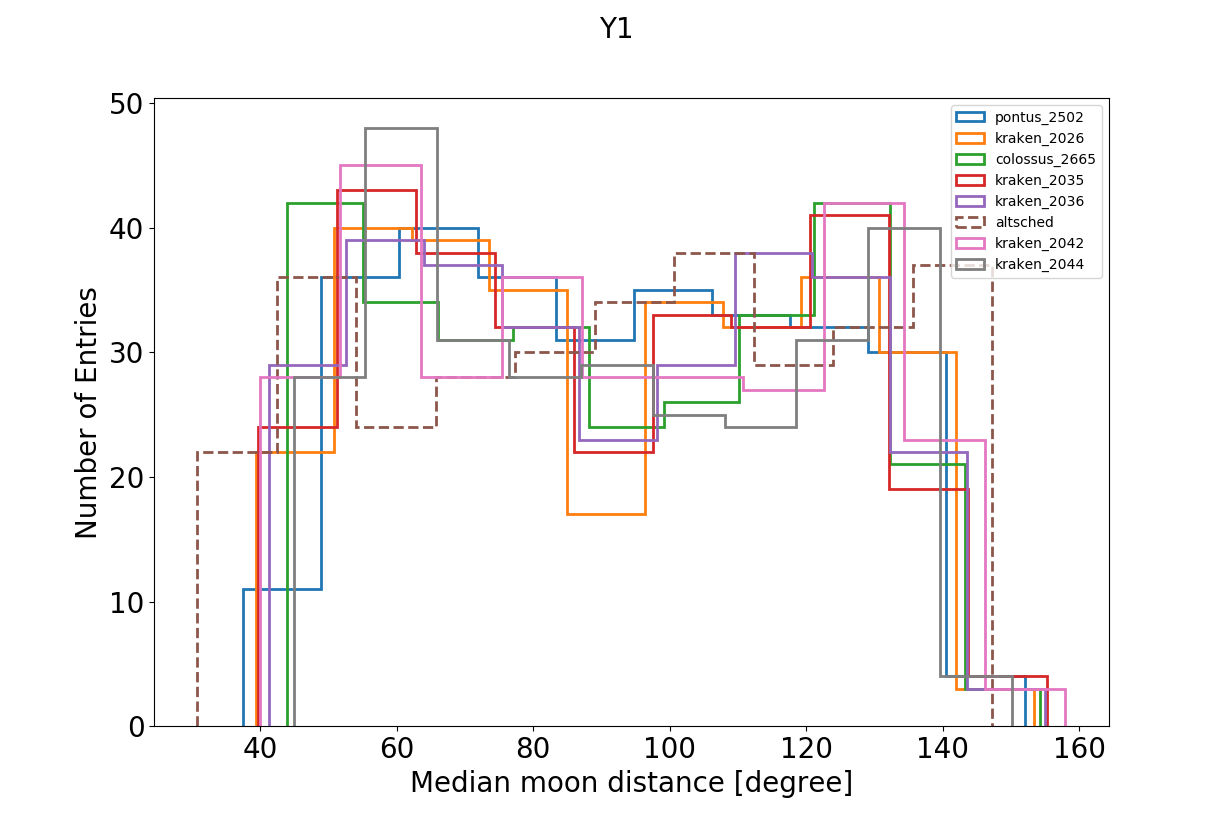
\includegraphics[width=0.6\textwidth]{opsim_vs_altsched/moon_distance.png}
    \caption{Median Moon distance (first year of the survey) for some of the observing strategies considered in this work.}\label{fig:moondist}
    \end{center}
\end{figure}


Finally other differences between the two schedulers include:
\begin{itemize}
\item{DDF} : DDF mini-surveys are not implemented in a coherent way in \altsched. A one hour slot per observing night is allocated to DDF observations but no filter sequence/observations performed during that time.\footnote{This corresponds to versions of the code used to perform the simulations considered in this note. An ongoing work initiated during the LSST Cadence Hackathon (17-19 September 2018; Flatiron Institute, New York, NY) by Daniel Rothchild and Philippe Gris aims at including DDF mini-surveys in a coherent way in \altsched.}
\item{Uncovered area}:  the North Ecliptic Spur, the North Galactic Pole and the South Celestial Pole are not observed by \altsched~.
\item{Galactic Plane}: the Galactic plane is observed by \altsched~in the same way as the WFD survey.

\end{itemize}

A way to quantify the impact of these differences on the main survey (in terms of cadence, filter allocation, ...) would be to ''fake'' these observations (ie allocate time for it with no realistic visit sequence).
